\chapter{Composizione fotografica}
\label{composizione_fotografica}
Esistono diversi fattori che dovrebbero essere tenuti in considerazione quando si vogliono catturare fotografie di qualità professionale. Alcuni dei più noti sono la luce, l'esposizione, la messa a fuoco, l'apertura, la scelta delle lenti. Fra questi, però, esiste un aspetto di cui raramente si discute: la composizione o \textit{image layout}.

\section{Cos'è la composizione fotografica}

Con composizione fotografica si intende disposizione strategica e calcolata degli elementi all'interno dell'immagine. Questo è un fattore determinante del modo in cui percepiamo e trasmettiamo il contenuto visivo di uno scatto. La composizione \textbf{governa il flusso di informazione}, dirige lo sguardo dell'osservatore verso determinati punti di interesse, influenza profondamente la nostra comprensione e \textbf{risposta emotiva} di fronte ad una immagine. Lo scopo ultimo di un fotografo dovrebbe essere quello di produrre una fotografia che sia visivamente piacevole e che allo stesso tempo possa trasmettere un messaggio, una storia, un sentimento. Questo risultato può essere ottenuto tramite un attento posizionamento del soggetto all'interno dello scatto e degli elementi attorno ad esso. 

Esistono diverse linee guida ampiamente accettate in ambito fotografico professionale come buone convenzioni da seguire per comporre uno scatto di qualità. Di seguito se ne discutono alcune delle più importanti. Si analizzeranno più nel dettaglio tutte le regole di composizione trattate con ulteriori immagini di esempio quando si andranno a introdurre i datasets utilizzati per svolgere il task di classificazione (Capitolo \ref{datasets}). 

% --------------------------------------
% ROT
%---------------------------------------
\subsection{Regola dei terzi}
\label{rot}
La regola dei terzi (RoT, \textit{rule of thirds}) divide l'immagine in una griglia di tre righe e tre colonne, per un totale di nove blocchi di ugual dimensione. L'idea è quella di \textbf{posizionare il soggetto} o gli elementi principali della fotografia, i punti focali, lungo le linee divisorie o \textbf{nei punti di intersezione} fra esse (Figura \ref{fig:rule_of_thirds}), che sono considerati i più armoniosi e visivamente interessanti per l'occhio umano.

\begin{figure}[ht]
    \centering
    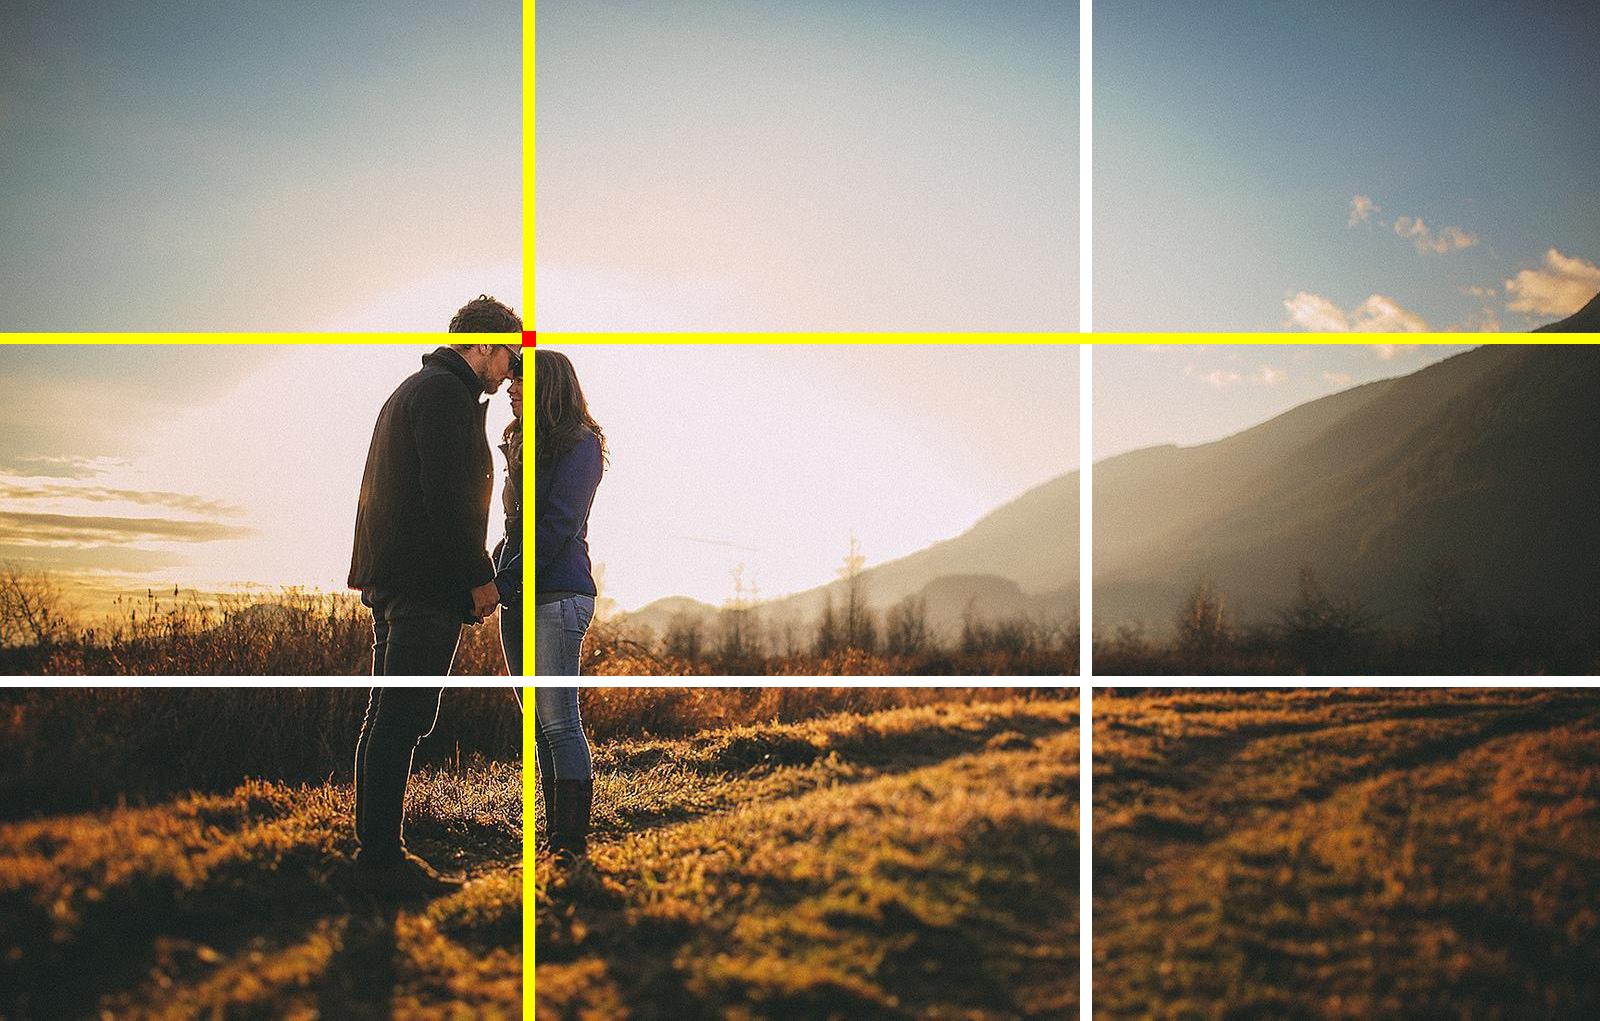
\includegraphics[width=0.7\textwidth]{Immagini/Introduzione/rot.png}
    \caption{Un esempio di regola dei terzi. I due soggetti sono posizionati lungo una delle linee guida, e il punto focale dello scatto si trova sull'intersezione di due di esse.}
    \label{fig:rule_of_thirds}
\end{figure}

Posizionare il soggetto in una di queste posizioni, piuttosto che al centro dell'immagine, conferisce un maggiore senso di \textbf{equilibrio, naturalezza}, aiuta a \textbf{guidare lo sguardo} dell'osservatore \textbf{verso i punti di interesse} principali della foto. Inoltre, la RoT può aiutare a dare un senso di profondità, di movimento, dinamismo, introduce un elemento di interesse ulteriore che aiuta ad elevare gli scatti.

% --------------------------------------
% Leading Lines
%---------------------------------------
\subsection{Leading Lines}
\label{leadinglines}
Un'altra tecnica spesso utilizzata da fotografi professionisti in ambito di composizione è quella delle \textit{leading lines}. Le leading lines sono delle vere e proprie \textbf{linee che guidano l'occhio dell'osservatore attraverso l'immagine} e verso il soggetto dello scatto o un altro punto di interesse che si vuole mettere in risalto. Possono essere linee reali o immaginarie, date dal posizionamento di fiumi, recinzioni, binari ferroviari, strade, linee architettoniche, orizzonti, alberi e altro.

\begin{figure}[b]
    \centering
    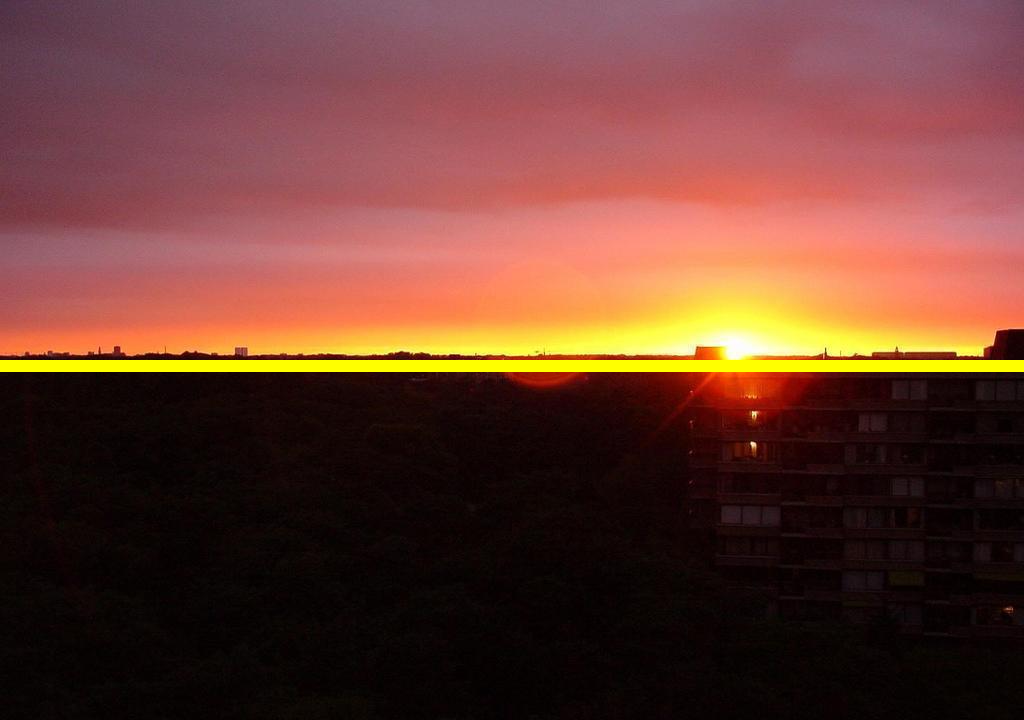
\includegraphics[width=0.3\textwidth]{Immagini/Introduzione/sunset_horizontal.png}
    \quad
    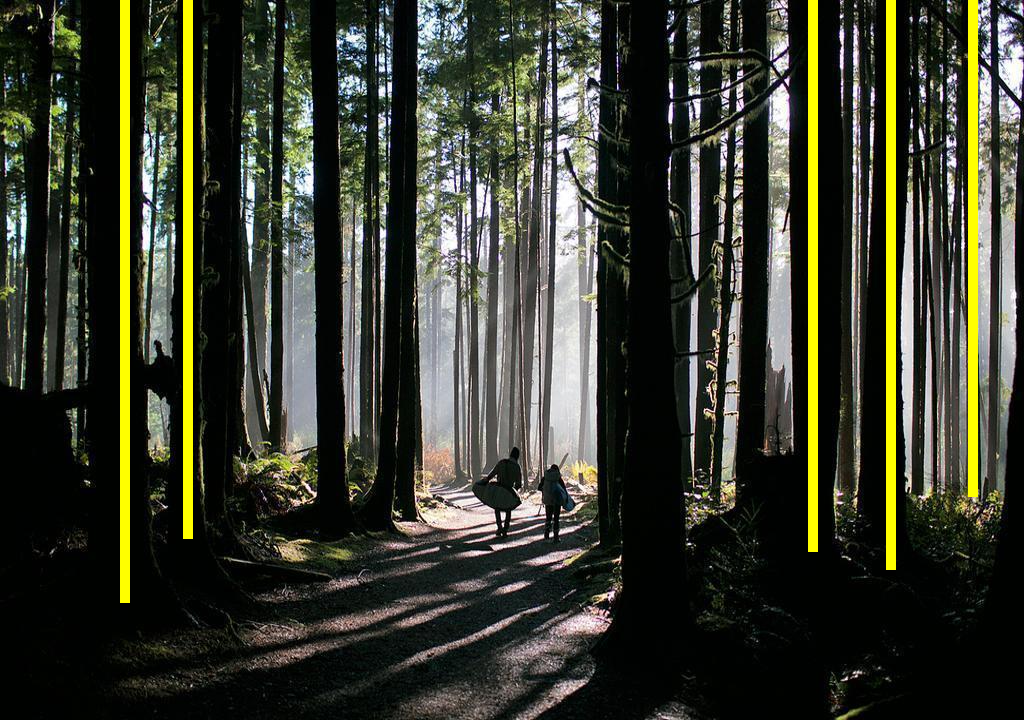
\includegraphics[width=0.3\textwidth]{Immagini/Introduzione/vertical.png}
    \quad
    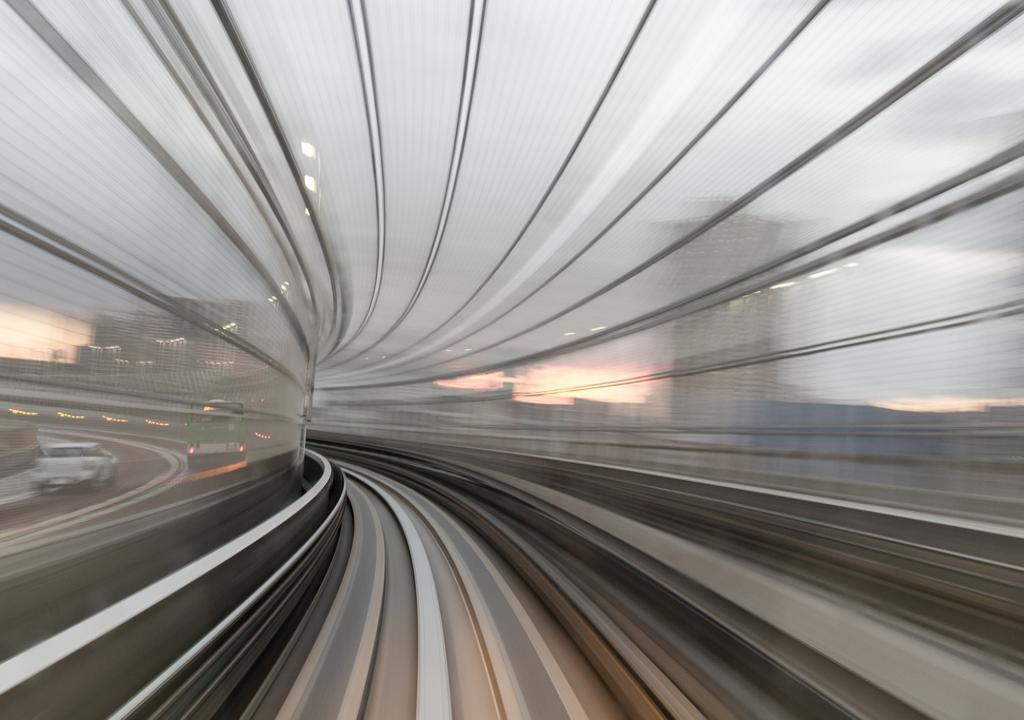
\includegraphics[width=0.3\textwidth]{Immagini/Introduzione/curved2.jpg}
    \caption{Esempi di leading lines orizzontali, verticali e curve, rispettivamente.}
    \label{fig:leading_lines}
\end{figure}

Possiamo distinguere diversi tipi di leading lines, ciascuna delle quali può trasmettere diverse sensazioni nel subconscio dell'osservatore:
\begin{itemize}
    \item Orizzontali: inconsciamente siamo soliti ad analizzare le immagini linearmente, da sinistra verso destra. Per questo motivo, linee orizzontali possono dare un senso di \textbf{conforto, stabilità, tranquillità}. Alcuni esempi possono essere orizzonti, file di alberi, linee costiere. Possono anche individuare simmetrie all'interno dell'immagine, come una montagna specchiata sulla superficie piatta di un lago, creando armonia e bilanciamento.
    \item Verticali: in natura e nel mondo urbano, linee verticali spesso si presentano sotto forma di alberi e alti edifici. Per questo motivo, al contrario del caso precedente, elementi verticali possono indurre una sensazione di sopraffazione, l'occhio è spinto a seguire tanti percorsi in maniera non lineare. Inoltre possono trasmettere \textbf{forza, crescita, potenza}.
    \item Curve: possono guidare lo sguardo in modo più morbido e naturale, creando un senso di \textbf{flusso, dinamismo, movimento}, che è difficile da riprodurre in scatti statici. Includono fiumi, sentieri, strade, curve architettoniche. In natura scarseggiano, spesso vengono accentuate artificialmente dall'utilizzo di lenti grandangolari.
\end{itemize}
Altri tipi di leading lines possono essere diagonali o convergenti, a formare un forte punto focale, come dei binari che convergono in lontananza.

\vspace{7mm}
\begin{figure}[!h]
    \centering
    \subcaptionbox{}{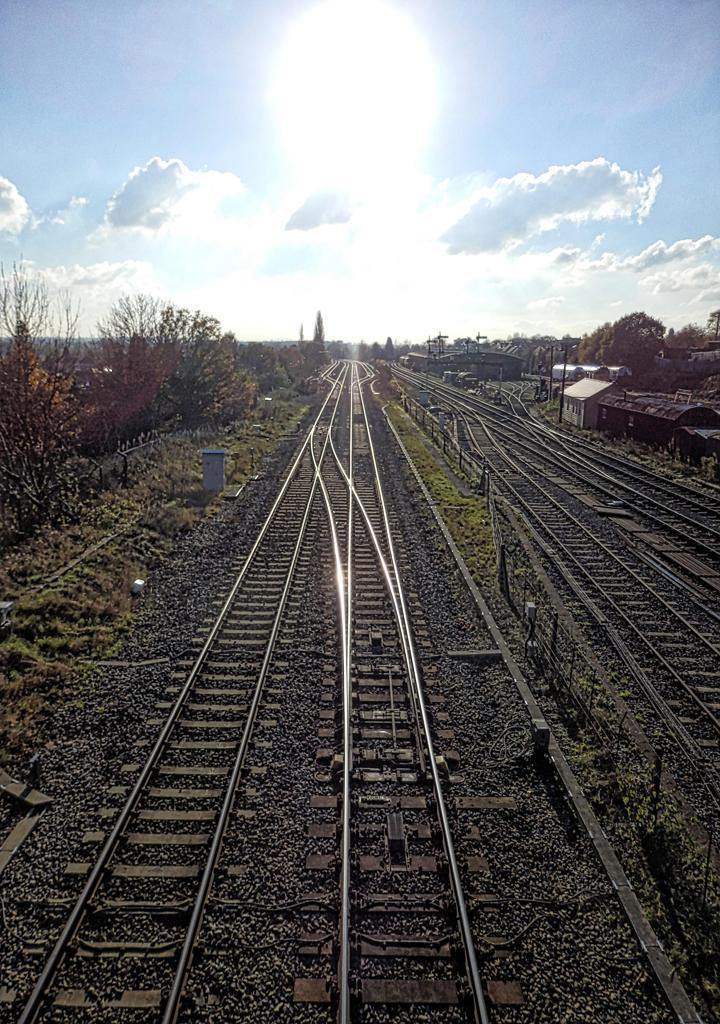
\includegraphics[height=50mm]{Immagini/Introduzione/convergenti.jpg}}
    \subcaptionbox{}{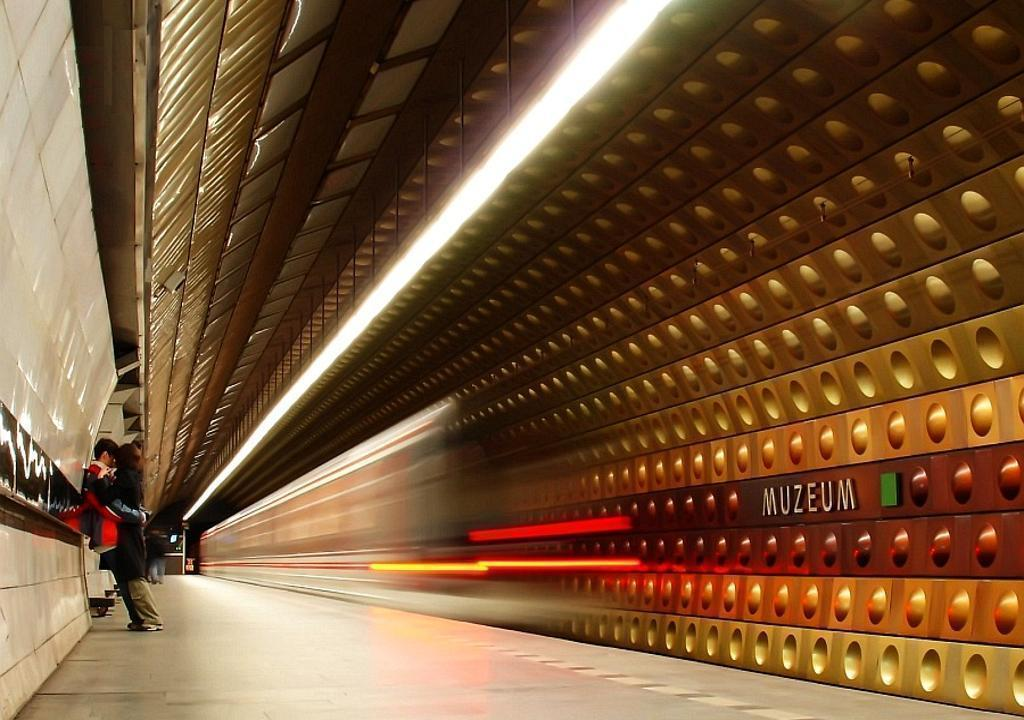
\includegraphics[height=50mm]{Immagini/Introduzione/diagonal.jpg}}
    \caption{Esempio di (a) leading lines convergenti, corrispondenti con l'unirsi dei binari all'orizzonte (b) leading lines diagonali.}
    \label{fig:diagonal}
\end{figure}

% --------------------------------------
% Forme e patterns
%---------------------------------------
\subsection{Forme e patterns}
Un'altra tecnica di composizione dello scatto è quella relativa alla forma dei soggetti e la presenza di \textit{patterns}. Posizionare la camera in modo da esaltare la \textbf{ripetizione di oggetti di struttura simile} permette di creare effetti visivi interessanti, accattivanti, di forte impatto (Figura \ref{fig:shape_patterns}b.). Anche effettuare lo scatto da angoli appositi che \textbf{accentuino delle forme} ben precise, come quella triangolare, possono dare più personalità all'immagine (Figura \ref{fig:shape_patterns}a.).

\begin{figure}[h]
    \centering
    \subcaptionbox{}{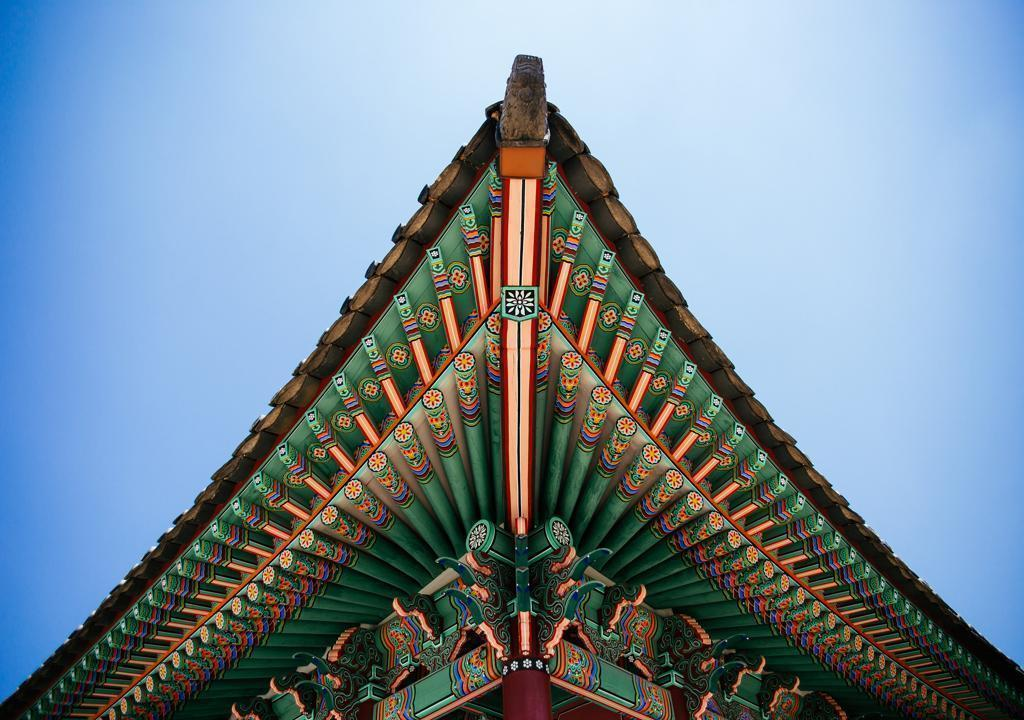
\includegraphics[height=45mm]{Immagini/Introduzione/triangle.jpg}}
    \quad
    \subcaptionbox{}{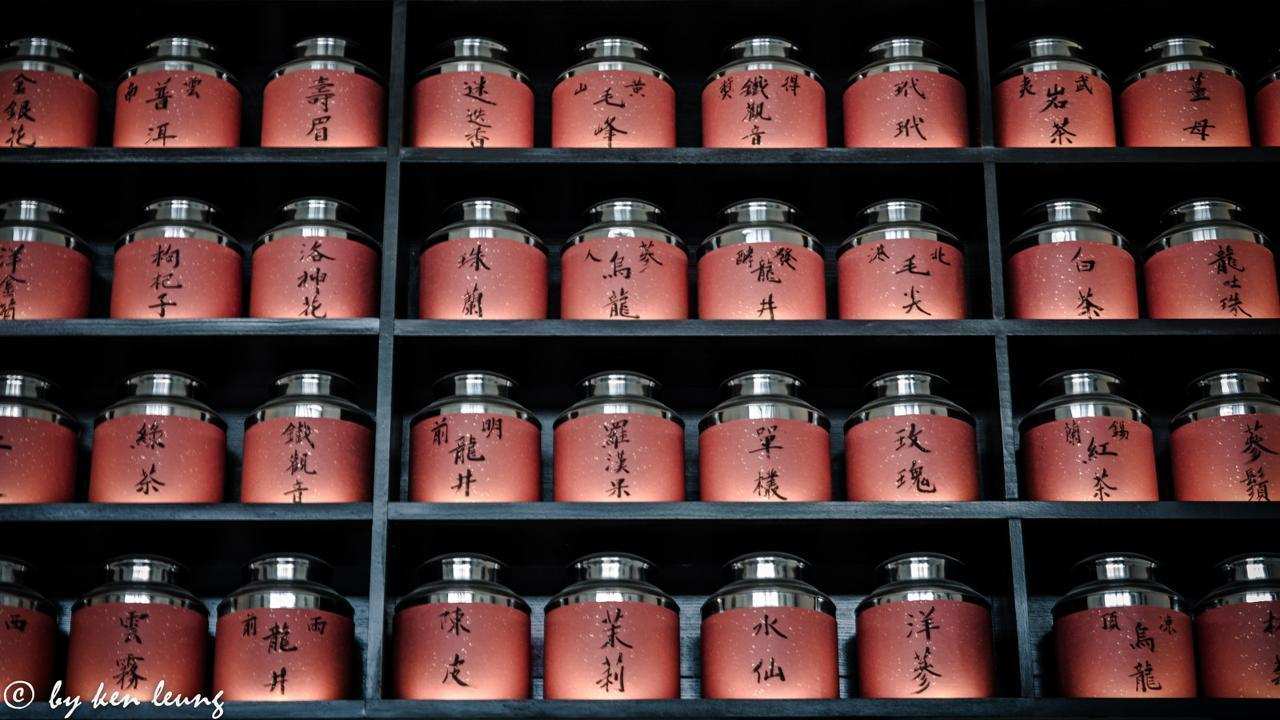
\includegraphics[height=45mm]{Immagini/Introduzione/pattern.jpg}}
    \caption{Esempi di (a) un soggetto triangolare (b) un pattern}
    \label{fig:shape_patterns}
\end{figure}

\section{Classificare la composizione}
I fotografi professionisti sfruttano elementi geometrici basilari come punti, linee, forme, per guidarli nella composizione delle immagini. Nonostante ciò, a causa della grande varietà di disposizioni, forme, colori dei soggetti, molti diversi elementi geometrici appaiono nelle fotografie. Per questo motivo, \textbf{determinare} la regola di \textbf{composizione rilevando} direttamente \textbf{gli elementi geometrici} dell'immagine \textbf{non è un approccio realistico}. È necessario avere una comprensione delle foto nella loro interezza per poterne determinare la composizione in maniera affidabile.

Ci sono stati approcci \cite{fuzzy2012} che utilizzano algoritmi convenzionali nell'individuare la classe di composizione delle immagini, sfruttando approcci che determinano quanto siano "ovvi" gli elementi di geometria e di colore nell'immagine, quanto siano prevalenti nel percepire lo scatto. Questo, però, risulta insufficiente nel classificare la composizione: un soggetto umano considera l'importanza contestuale di ciascun elemento tanto quanto la sua rilevanza all'interno dell'immagine. Ad esempio, nella Figura \ref{fig:curved_fence}, l'elemento che risulta essere più ovvio studiando caratteristiche di basso livello, come l'intensità di colore, è lo stacco fra il cielo e il terreno, l'orizzonte. Nonostante ciò, guardando l'immagine, l'elemento che a un utente umano salta immediatamente all'occhio è la staccionata, che può coincidere con una leading line curva, e quindi classificare lo scatto con tale composizione.

Per questo motivo, l'approccio preferenziale è quello di imparare features discriminanti a partire da un grande numero di immagini annotate da esseri umani, piuttosto che delle caratteristiche studiate manualmente, ad hoc. Di conseguenza, negli esperimenti condotti durante lo stage che verranno esposti successivamente, sono stati utilizzate tecniche di \textit{deep learning} sui datasets KU-PCP \cite{KU-PCP} e LODB \cite{LODB}, le cui origini e caratteristiche saranno approfondite nei Capitoli \ref{sota} e \ref{datasets}.


\begin{figure}[b] 
    \centering
    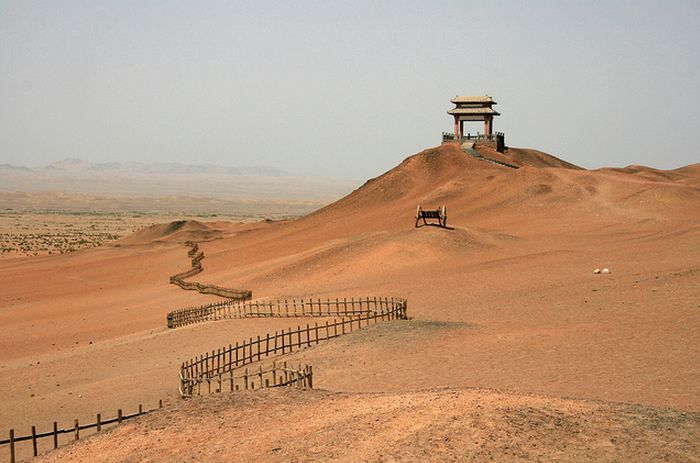
\includegraphics[height=60mm]{Immagini/Introduzione/Stories - Lonely Planet.jpeg}
    \caption{Le leading lines curve implicite date dalla forma della staccionata risultano più importanti all'occhio umano rispetto alla separazione fra cielo e terreno.}
    \label{fig:curved_fence}
\end{figure}

Inoltre, per il task di classificazione, in questa relazione si utilizzeranno features prodotte tramite un modello addestrato con la tecnica della \textbf{self-supervision}. Negli ultimi anni, specialmente dopo il 2020, c'è stata una forte accelerazione nella ricerca riguardante i metodi di \textit{self-supervised learning}, che ha portato alla nascita di DINOv2 \cite{dinov2}, un foundational model di MetaAI che ha prodotto risultati molti promettenti nell'ambito della classificazione della semantica delle immagini, e non solo. Le sue caratteristiche saranno meglio esplorate nel Capitolo \ref{ssl}. L'analisi proposta nasce dalla curiosità di valutare le prestazioni di DINOv2 sul task presentato e verificare se le features che esso estrae possano essere utilizzate per problemi più di alto livello rispetto al riconoscimento dei soggetti, come appunto l'analisi degli elementi geometrici e spaziali nell'immagine.

Da notare è che quello della composizione è un problema di classificazione \textit{multilabel}, una foto potrebbe presentare l'utilizzo di più tecniche compositive, come illustrato nella Figura \ref{fig:multilabel_examples}.

\vspace{7mm}

\begin{figure}[t] 
    \centering
    \subcaptionbox{}{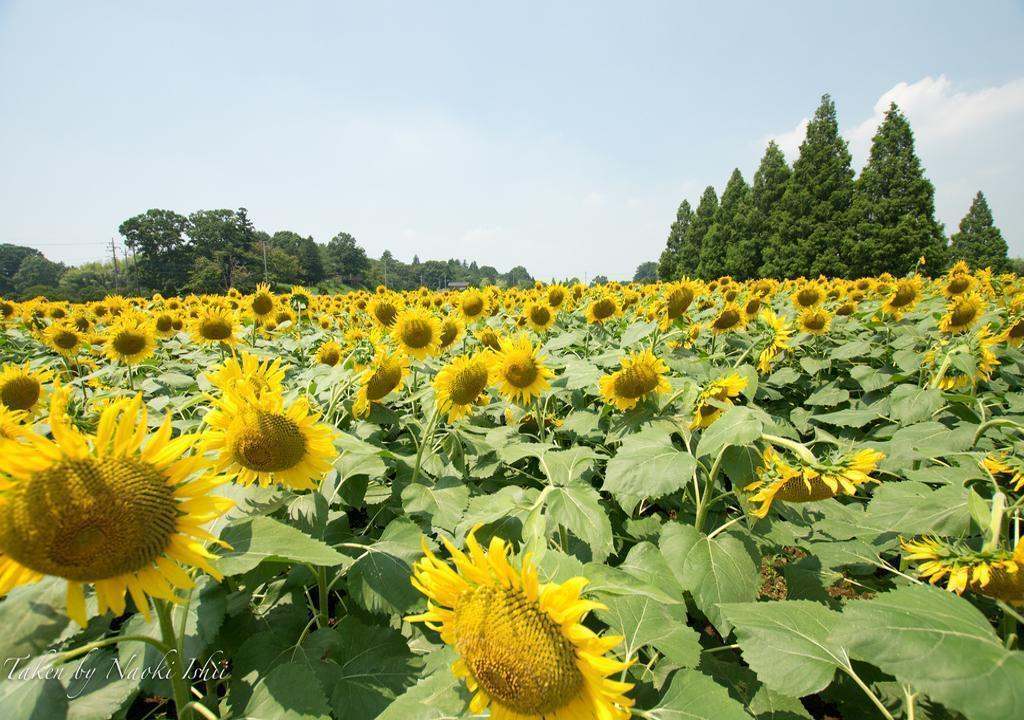
\includegraphics[height=35mm]{Immagini/Introduzione/horizontal_pattern.jpg}}
    \subcaptionbox{}{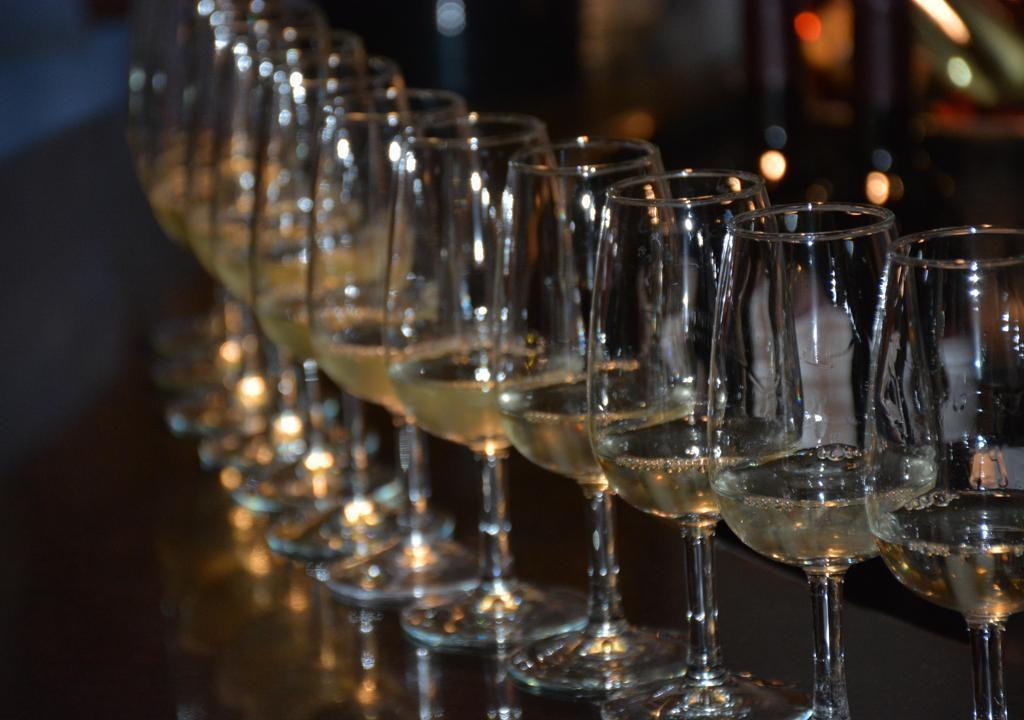
\includegraphics[height=35mm]{Immagini/Introduzione/pattern_curve.jpg}}
    \subcaptionbox{}{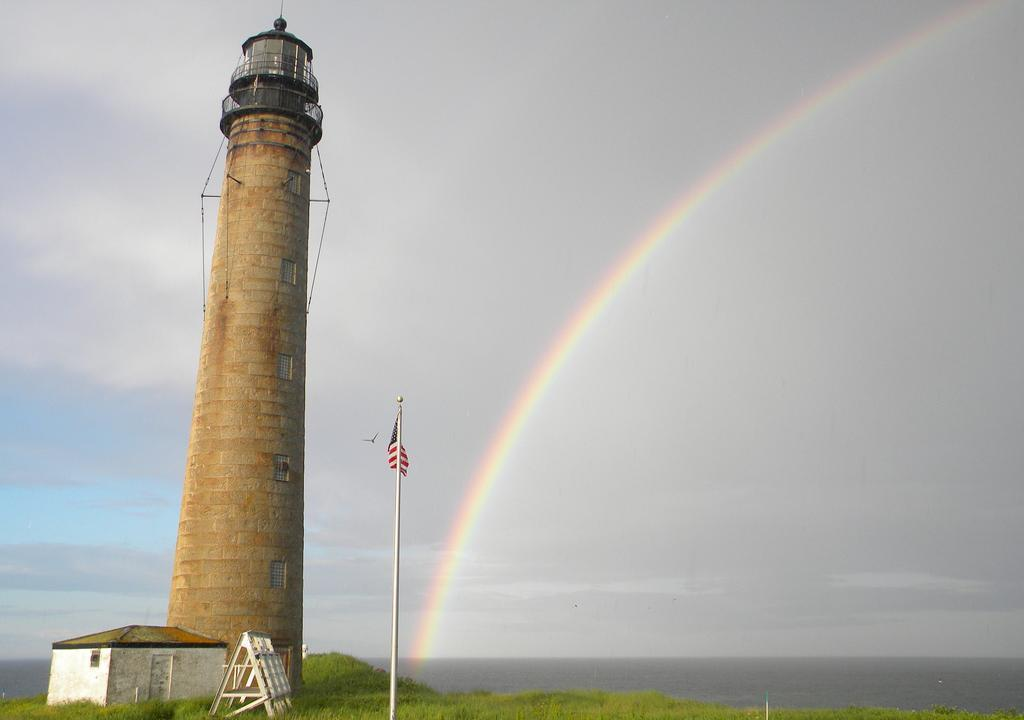
\includegraphics[height=35mm]{Immagini/Introduzione/vertical_rot.jpg}}
    \caption{Immagini classificabili con più tipi di composizione: (a) horizontal leading line e pattern, (b) curva e pattern, (c) verticale e RoT}
    \label{fig:multilabel_examples}
\end{figure}


\section{Scopo e utilizzi pratici}
Nonostante l'importanza che la composizione fotografica detiene nel migliorare e nel determinare la qualità estetica di uno scatto, questo è un aspetto che raramente viene considerato, soprattutto da parte di fotografi amatoriali e inesperti. È per questo motivo che la creazione di tools che possano assistere l'utente nel compito di comporre abilmente gli scatti potrebbe risultare utile. Pensiamo alle app Fotocamera dei nostri smartphones: e se queste avessero la capacità di guidarci nel produrre scatti migliori oltre il semplice allineamento dell'orizzonte? L'arte fotografica sarebbe molto più accessibile anche per chi non ha necessariamente le basi tecniche che ha un veterano nel settore. 

Uno strumento utile in ambito istruttivo per un giovane fotografo potrebbe essere quello di sottoporre ad un sistema automatizzato una immagine statica, già scattata, allo scopo di ottenere un insieme di dettagli e tecniche utilizzate per produrla, da cui imparare. Alternativamente, potrebbe essere usato come fonte di critica dei propri scatti e come punto di riflessione su come poterli migliorare, anche per chi ha già esperienza nel campo. 

Un altro spunto potrebbe essere quello di introdurre questo tipo di aiuto in software di editing fotografico (\textit{Photoshop}, ma anche video editing come \textit{Adobe Premiere}), in modo che possa guidare operazioni come il \textit{cropping} o la rotazione di un'immagine, suggerendo quale sia l'approccio migliore per ottenere un risultato che rispetti le linee guida di composizione, per una qualità estetica migliorata.   

Oltre all'aspetto prettamente fotografico, potremmo anche pensare di estendere questo studio alla grafica e al design. Sarebbe importante l'introduzione di uno strumento che assista il designer nell'impaginazione degli elementi di una grafica, seguendo le stesse regole di leading lines, RoT, forme, patterns, e altri. In ambito di marketing potrebbe aiutare nel suggerire come guidare l'attenzione degli utenti verso gli elementi che si vogliono evidenziare in una inserzione pubblicitaria. 

In ambito ricreativo, un tool come quello discusso potrebbe aiutare l'artista a meglio comprendere come trasmettere determinate sensazioni tramite le sue creazioni, esponendogli quale sia la migliore costruzione dell'immagine in base al sentimento che egli vuole ritrarre. Facendo un rapido riferimento ai miei interessi personali, la parte più complicata del produrre un render tramite Blender non è sempre il modellare la scena nei suoi aspetti più tecnici e geometrici, come si potrebbe pensare, bensì il come posizionare la camera nella scena 3D in modo che il risultato finale sia armonico e valorizzi la propria visione artistica.

Un primo passo nel raggiungere lo sviluppo di software che possano guidare l'esperienza del fotografo, dell'artista, del designer, è quello di essere in grado di riconoscere gli elementi compositivi degli scatti, che portano una grande influenza sul valore estetico, e non solo, delle immagini in tutti i settori menzionati.

\section{Outline}
Questa relazione si concentrerà su uno studio dello stato dell'arte nell'ambito della classificazione della composizione delle immagini, nel Capitolo \ref{sota}. Successivamente si presenterà una panoramica sull'evoluzione delle tecniche di self-supervision che hanno portato alla nascita di DINOv2 nel Capitolo \ref{ssl}. Nel Capitolo \ref{metodo} si descriverà il metodo utilizzato per ottenere i risultati esposti nel Capitolo \ref{risultati}. La descrizione dei dataset usati si trova al Capitolo \ref{datasets}.
Infine, nel Capitolo \ref{conclusioni} si faranno delle considerazioni finali sui risultati prodotti e su possibili sviluppi e altre strade da esplorare in futuro.